PocketShelf is an IOS/ Android based mobile application which allow user to keep their items in available space, which is previously created by user. We called it "PocketShelf" because, basically one is carrying all the shelf inside his/her pocket, like s/he can find his/her item just in a click. Not only that s/he can add an item in the app and app will decide where to keep that item, and it will ask some image of that item after which they can put that item on the given shelf and can forget where they kept it. All the remembering things will be done by the app, on top of it, our app will allow user to see the actual image of that item, so that the user can know that the item s/he is looking for is the exact item on the shelf before they grab it which will save their time and effort. Based on the items that can be added to the app, our application have different versions. 


\subsection{Features \& Functions}
"PocketShelf" is an inventory app, that can keep track of any item that user wants. We used Augmented reality as our key feature of the application. Where user can see the item before s/he approach to grab it. Which might be helpful in the sense that it will save the user effort and time spent, it s/he known that they are getting the right thing. Our app not only keep track of the item but able to sort the items based on the expiration dates and can notify the user if the item is expiring soon. Time frame to notify user can be pre- defined by the user at the time of its entry. Our app use the online database to save every entry by the user and had to be encrypted before it goes to the database, all the data had to flow through the server. So, user have to be online to be able to use the app. We had PIN protection as an extra feature on the app, where if the user want not to show the item location to other user using the same app on same device. Which we found cool feature if the user wants to secure his/her valuable items somewhere in the shelf.


\subsection{External Inputs \& Outputs}
 Initial version of PocketShelf is vary basic version of inventory app, which is fully based on the user input rather then machine learning's predictions. Each and every input should go through user.User can scan the bar code of the item to be stored(optional), user have to give unique name to the item to be store, user can add some notes about the item in item description field, user must dive the quantity of item to be stored in the shelf, it can be one or more. If the item have expiration date and user want to keep track of the expiration of any item on the shelf, during entry they can specify the expiration date and enable the notification before the specified date. If user does not want other user to see the location of the item, s/he can enable PIN protection for the location. User must add the picture of the item to be stored before adding to the database. Once user provide all valid input, user can press add button after which app will give the available location with a QR-code, user can save the QR-code for his record. Later if the user wants to retrieve some item, s/he can scan the QR, where the app will show the picture of the item up on the QR, to help user to able to identify the item. Once user pick the item S/he should input quantity picked from the location. If the location is PIN protected, during QR scan app will ask PIN to verify the user before reveling the item picture and item location. 
\pagebreak

\subsection{Product Interfaces}
These are some of the user interface. Where Home screen is shown as soon as application is launched, if user wants to add item app will launch adding item screen and so on. We had implemented our interface in such a way that even a color blind person can easily use our app.
\\Home Screen
\begin{figure}[hbt!]
                	\centering
                   	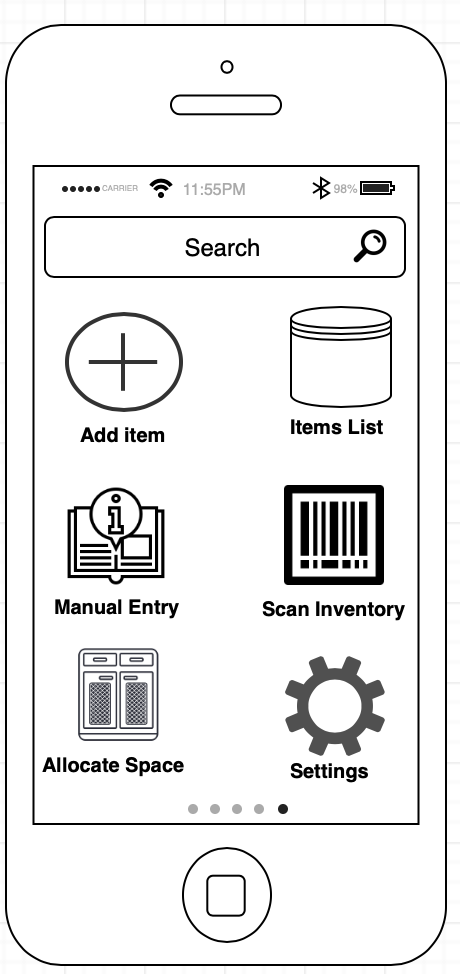
\includegraphics[width=0.19\textwidth]{images/home}
                    \caption{Home Screen}
                \end{figure}

Adding Item.
\begin{figure}[hbt!]
                	\centering
                   	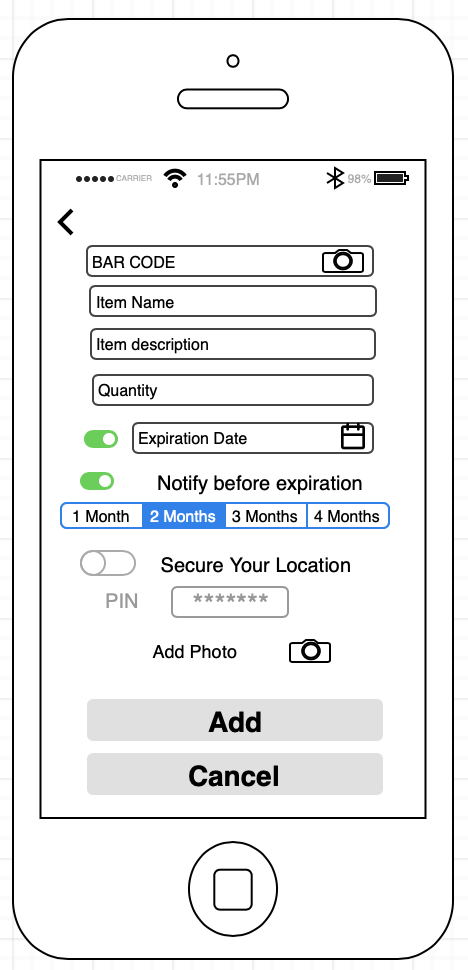
\includegraphics[width=0.19\textwidth]{images/adding}
                    \caption{Adding item}
                \end{figure}
                
\pagebreak
Product Search.
\begin{figure}[hbt!]
                	\centering
                   	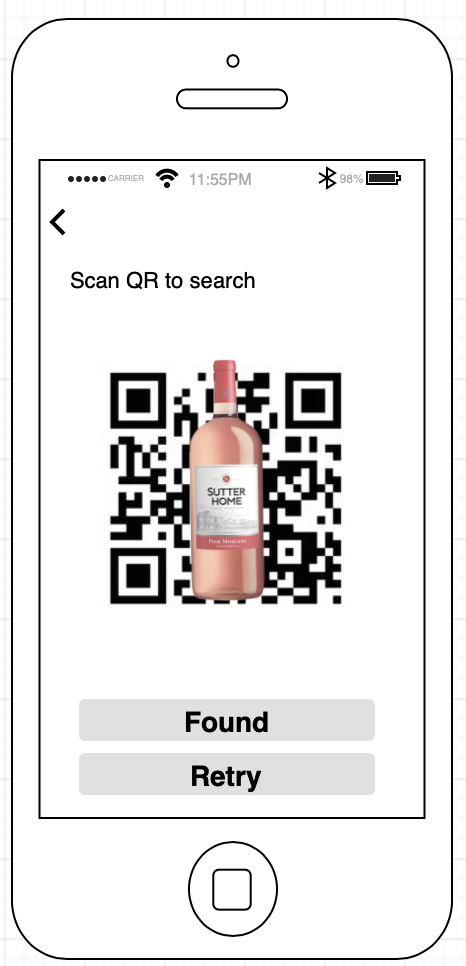
\includegraphics[width=0.19\textwidth]{images/search}
                    \caption{Product search using QR}
                \end{figure}
\\Product Found.
\begin{figure}[hbt!]
                	\centering
                   	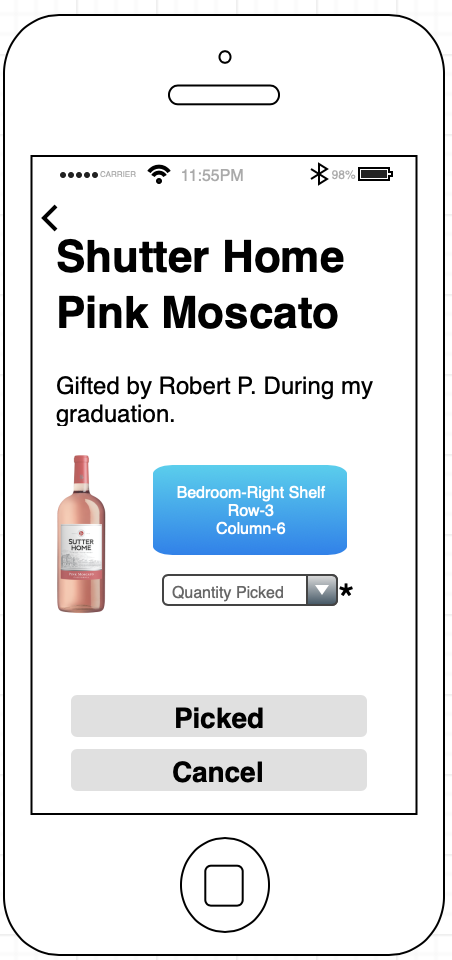
\includegraphics[width=0.19\textwidth]{images/pick}
                    \caption{Picking product once found}
                \end{figure}
\pagebreak
\\Adding New Shelf.
\begin{figure}[hbt!]
                	\centering
                   	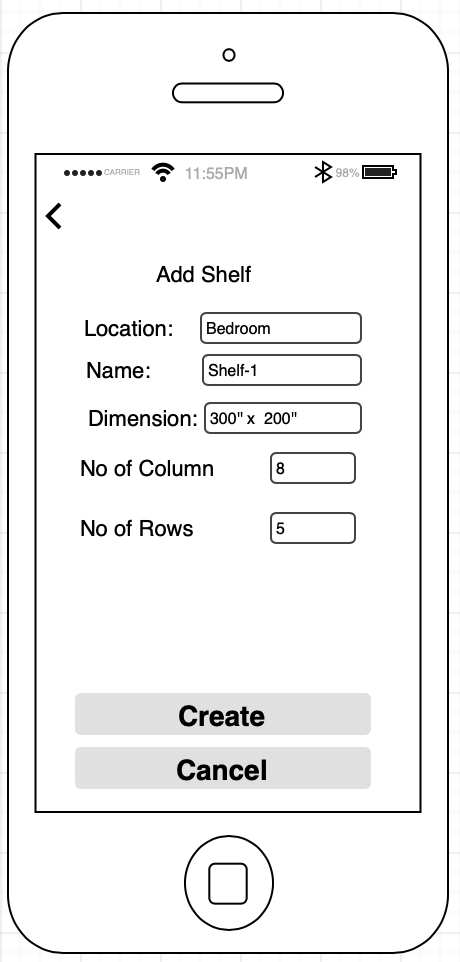
\includegraphics[width=0.19\textwidth]{images/shelf}
                    \caption{Adding Shelf}
                \end{figure}
